\documentclass{article}

\usepackage[T1]{fontenc}
\usepackage{amsmath, amssymb}
\usepackage{ngerman}
\usepackage{graphicx}
\usepackage{tabularx}
\usepackage{mathptmx}
\usepackage[scaled=.92]{helvet}
\usepackage{courier}
\usepackage{float}

\begin{document}

\parindent0cm % verhindert das Einrücken von Absätzen 

% Hier wird die Titelseite gebastelt
% Zuerst wird die Seite auf empty eingestellt, das heißt sie hat keine 
% Seitenzahl und auch keine Kopf- bzw. Fußzeile
\thispagestyle{empty}

% Der Titel wird zentriert in fetter riesiger Schrift gesetzt.

\begin{center}
\begin{Huge}
\textbf{Bachelorprojekt Informatik \\ \vspace{0.2cm}
CS3701-KP05\\ \vspace{2.5cm}
Institut für Telematik\\ \vspace{0.2cm}
Wintersemester 2025/26\\\vspace{2.5cm}
Entwicklung einer Android-App zur mobilen
Überwachung der H0-Modellbahn}\vspace{1.5cm}
\end{Huge}

% Weiter in großer Schrift

\begin{huge}
Thorben Heinz, 756972 \\
Yannic Biallas, 771216 \\
Lübeck, \today 

\textbf{Leitung:} Prof. Dr. Stefan Fischer

\textbf{Mitarbeiter:} Ingrid Schumacher, Dipl.-Inf.\\
Klaus-Dieter Schumacher, Dipl.-Inf. 
\end{huge}

\end{center}

% Inhaltsverzeichnis

\setcounter{page}{0}

\newpage 
\pagenumbering{roman} 


\tableofcontents 

\newpage

% Start der eigentlichen Arbeit

\setcounter{page}{0}
\pagenumbering{arabic} 

\section{Ziel der Arbeit}
Die Android App \textbf{MobileTrainTestsoftware} dient als mobile Erweiterung der Leitstelle und ergänzt die auf den Steuerrechnern installierte Testsoftware.
Die momentan auf den Steuerrechnern installierte Testsoftware hat den Nachteil, dass zwei Personen zum Testen der jeweiligen Ebene notwendig sind.
Unmittelbar nach dem Schalten einer Komponente ist diese bereits geschaltet und es ist nicht leicht erkennbar, ob dies problemlos abgelaufen ist.
Mit der von uns entwickelten Android App MobileTrainTestsoftware kann eine geschaltete Komponente direkt beobachtet werden, da die Nutzung der App mobil möglich ist.

\subsection{Anforderungen}
Zu Beginn des Projektes wurde von unserer Auftraggeberin Frau Schumacher festgelegt, welche Anforderungen unsere App erfüllen soll.
Die zu entwickelnde App soll alle Ebenen der Modelleisenbahnanlage darstellen und steuern können.
Weichen und Streckenblöcke sollen mit dem Gleisplan dargestellt sein und durch interaktives Feedback steuerbar sein.
Außerdem soll die App über eine angenehme und moderne UI verfügen.

\section{Einleitung}\label{einleitung}
Hier folgt noch eine Einleitung zu der Modelleisenbahnanlage.


\section{Analyse bisheriger Technologien}
\subsection{Netzwerkkommunikation}
Die Kommunikation wird in der Modelleisenbahnanlage auf unterschiedliche Weise umgesetzt.
Dabei befinden sich alle Geräte im selben Netzwerk, über welches die Kommunikation läuft.

Zum einen gibt es die Leitstelle (Pi400). 
Sie kommuniziert mit auf der Anlage verteilten Steuerrechnern (RPi4) zum Ändern der Zustände von Weichen oder Streckenblöcken.
Die Leitstelle sendet dazu zunächst die eigene IP-Adresse per UDP-Broadcast an alle, im Netzwerk vorhandenen, Steuerrechner. 
Gleichzeitig wird ein Thread zum Annehmen einer TCP-Verbindung zu den jeweiligen Steuerrechnern gestartet. 
Jede TCP-Verbindung kann zum Senden von Informationen (neue Komponentenkonfiguration) oder dem Empfang von Zuständen der Komponenten verwendet werden. 
Dazu läuft jede TCP-Verbindung in einem eigenen Thread. Wenn eine definierte Anzahl Steuerrechner eine TCP-Verbindung zu der Leitstelle aufgebaut haben, wird ein Initialzustand (für Weichen und Streckenblöcke) an alle Steuerrechner gensendet. 
Eine Zustandsänderung einer Komponente wird per UDP übertragen und es wird auf eine Antwort des zuständigen Steuerrechners gewartet. 
Nachzulesen ist dies in der main.py und Network\_new.py in der Leitstellen Software.
Die Steuerrechner wiederum warten auf einen ankommenden UDP-Broadcast der Leitstelle. 
Nachdem die UDP- und TCP-Sockets eingerichtet wurden, wird der UDP-Socket abgehört. 
Erfasst der Steuerrechner ein UDP-Broadcast, so baut der Steuerrechner eine TCP-Verbindung zu der IP-Adresse der Leitstelle auf, welche in der UDP Nachricht mitgesendet wird.
Wichtig ist, dass der Steuerrechner eine TCP-Verbindung zum Port 6005 öffnet.
Würde an der Leitstelle ein anderer Port für die TCP-Verbindung geöffnet, so könnte keine Verbindung hergestellt werden.
Die IP-Adresse muss für den Steuerrechner nicht im String der UDP-Nachricht enthalten sein, da diese schon im Daten-Paket vorhanden ist.
Somit erwarten die Steuerrechner als Verbindungsaufbau UDP-Nachricht keinen spezifischen String.
Der Steuerrechner des Lift-Blocks erwartet allerdings einen spezifischen String.
Wird dieser nicht gesendet, so baut er keine Verbindung auf. 
Über die aufgebaute TCP-Verbindung wird eine Nachricht mit dem erfolgreichen Verbindungaufbau an die Leitstelle zurückgeschickt. 
Anschließend wird die UDP-Verbindung vom Steuerrechner in einem eigenen Thread abgehört. 
Nachdem alles initialisiert ist, wird in die Main-Loop übergegangen, wo das jeweils älteste Element einer zuvor initialisierten Queue behandelt wird. 
Wird eine Nachricht via UDP empfangen, so wird in dieser Nachricht überprüft, ob der jeweilige Steuerrechner angesprochen wird. 
Sollte das nicht der Fall sein, wird die Nachricht verworfen. 
Sollte das Level dem Level des Steuerrechners entsprechen, so wird der Befehl in der Queue abgelegt. 
Nach der Ausführung des Befehls, wird mit Hilfe des Communicators eine Bestätigung der Ausführung über TCP an die Leitstelle zurückgesendet. 
Nachzulesen ist dies in \_\_main\_\_.py und communicator.py in der Software des Steuerrechners.



\section{Umsetzung der Android App}

\subsection{Planung der Android App und Entwicklungsschritte}
Nachdem die Anforderungen an unsere App festgelegt wurden, haben wir eine Einführung in die Modelleisenbahnanlage bekommen. 
Dabei haben wir uns die Gleispläne und die eingesetzten Geräte (Steuerrechner, Leitstelle, Tablet) angesehen.
Zu der Steuerrung via Steuerrechner haben wir mit direkten I2C Befehlen einige Weichen testweise über einen der Steuerrechner geschaltet.
Dies half uns, ein Verständnis für die Befehle und Schaltungslogik der Anlage zu bekommen.
Als Resultat haben wir einen Arbeitsplan entwickelt.

Im Vorhinein haben wir vereinbart, Schritte arbeitsteilig anzugehen.
Yannic entschied sich, die Gestaltung der App sowie das Frontend zu übernehmen, während Thorben die Netzwerkkommunikation und das Backend übernahm.
Der Arbeitsplan enthielt folgende Schritte:
\begin{enumerate}
    \item Bezeichnung der Weichen und Streckenblöcke auf der Anlage mit Etikitiergerät anbringen
    \item Skizze für den Aufbau der App entwickeln (Yannic)
    \item Analyse der vorhandenen Technologie und Kommunikationstechnologie der App festlegen (Thorben)
    \item Mockup der App erstellen (Yannic)
    \item Erstes Element der Anlage in Praxisversuch schalten (Thorben)
    \item Alle anderen Funktionen umsetzen (Yannic und Thorben)
    \item Front- und Backend zusammenfügen
    \item Iteration ab Punkt 6, falls der Auftraggeber nicht zufrieden ist
    \item Abgabe des finalen Produkts und Dokumentation
\end{enumerate}

Nach der Analyse der vorhandenen Technologien haben wir uns bezüglich der Netzwerkkommunikation zuerst Gedanken darüber gemacht, wie wir Nachrichten an Steuerrechner senden können.
Unsere erste Überlegung war, alle Steuerrechner einzeln direkt via SSH anzusprechen.
Allerdings wurde uns schnell bewusst, dass diese Idee nicht umsetzbar ist, da die Steuerrechner eine dynamsiche IP-Adresse haben.
Für eine direkte Kommunikation via SSH bräuchten wir die IP Adresse der jeweiligen Steuerrechner.

Nachdem wir diese Idee aufgegeben hatten, haben wir uns an eine Internetprotokoll basierte Kommunikation wie zwischen Leitstelle und Steuerrechner festgelegt.
Um einen ähnlichen Ansatz wie bei der vorhandenen Kommunikation zu verfolgen, war es nötig, die bereits vorhanden Umsetzungen zu analysieren.
Nachdem wir dies getan haben, haben wir in einem ersten Test versucht festzustellen, ob die Kommunikation auch mit einer Android App funktioniert.
Getestet haben wir dies zu Beginn mit einem einfachen Button, der lediglich eine einzige Weiche schaltet konnte.
Die Steuerrechner sind beim Testen zu Beginn abgestürzt, da unsere Testversion noch keinen TCP-Listener hatte.
Nachdem die Steuerrechner allerdings korrekt mit der Leitstelle verbunden ware, war es kein Problem eine UDP-Nachricht von einem zweiten Gerät neben der Leitstelle an die Steuerrechner zu senden.
Das Ergebnis dieses Tests war, dass wir ohne Initialisierung der Steuerrechner eine Weiche korrekt schalten konnten.
Nach diesem Ergebnis haben wir die grafische Benutzeroberfläche entworfen und an einer TCP-Listener-Methode gearbeitet.

\subsection{Netzwerkkommunikation}
Die Android App befindet sich im selben WLAN wie die anderen Komponenten der Modelleisenbahnanlage.
Dies ist das Netzwerk \textbf{eisenbahn}, welches aktiv ist, sobald dies an der Fritz-Box eingeschaltet ist.
Die App hat im Android-Manifest die Erlaubnis, Netzwerkkommunikation zu nutzen.

Zuerst wird ein TCP-Listener gestartet, der den TCP-Port 6005 abhört.
Sollte der TCP-Listener einen Verbindungsaufbau erfassen, so wird dieser in einem neuen Thread behandelt.
Dies ermöglicht, eine TCP-Verbindung mit mehreren Clients herzustellen.
In diesem Fall sind die Clients die Steuerrechner der jeweiligen Modellbahn Ebenen.
Anders als bei der Leitstelle warten wir nicht auf eine Verbindung zu allen Steuerrechnern der Anlage, sondern öffnen so viele Threads, wie Verbindungen eingehen.

Über einen Button links unten kann man steuern, ob ein Verbindungaufbau zu den Steuerrechnern erfolgen soll.
Beim Öffnen der App ist unsere App im Disconnected Modus, was auch auf dem Button angezeigt wird.
Möchten wir eine Verbindung herstellen, so aktivieren wir den Button.
Es erscheint der Text connecting und der Button ist orange.
Im Hintergrund wird nun eine Nachricht via UDP-Broadcast an alle Netzwerkgeräte im selben Netzwerk gesendet.
Die Nachricht enthält einen String und das zugehörige Datenpaket, in dem auch die IP-Adresse enthalten ist.
Der UDP-Broadcast läuft wie auch der TCP-Listener in einem eigenen Thread.

Sobald ein Steuerrechner den UDP-Broadcast entdeckt, so stellt er eine TCP-Verbindung mit der Android App auf Port 6005 her.
Der Button, der vorher noch connecting angezeigt hat, ist nun grün und zeigt verbunden an.
Der Steuerrechner sendet nach dem erfolgreichen Herstellen der Verbindung einen String mit der Ebene, die er steuert (Ebene 0,1,2).
Die nun verbundenen Steuerrechner warten jetzt auf Nachrichten der Android App.

Wird eine Aktion wie etwa das Schalten einer Komponente in der App durchgeführt, so wird ein String mit dem dazugehörigen Befehl an die Steuerrechner via UDP-Nachricht gesendet.
Alle Steuerrechner empfangen demnach die Nachricht aber wie bereits bei der Analyse der bereits vorhandenen Technologien beschrieben, verarbeiten sie nur Nachrichten, die für sie vorgesehen sind.
Sollte ein Befehl einem Steuerrechner zugehörig sein, so setzt er den Befehl um und antwortet mit einem Acknologement, welches eine Kopie des von der App gesendete Strings ist.
Unsere App empfängt den String des Steuerrechners mit dem TCP-Listener und zeigt das Ack an.

Soll die Verbindung mit den Steuerrechnern unterbrochen werden, so kann über den Button mit einem Klick die TCP-Verbindung zu allen Clients geschlossen werden.
Nach dem Klick auf den Button, ändert sich das Aussehen von grün und der Anzeige verbunden zu rot und Disconnected.



\subsection{Architektur der App}
In diesem Kapitel wird das technische Gerüst der App beschrieben. Da die Steuerrechner keine Zustandsrückmeldungen liefern, übernimmt die App die Rolle des alleinigen Zustandsverwalters („Single Source of Truth“). Um eine blockierfreie Bedienung zu gewährleisten, ist die Architektur konsequent auf Multithreading ausgelegt: Alle Netzwerkoperationen (UDP-Senden und TCP-Listening) laufen in dedizierten Hintergrund-Threads ab, um den Haupt-Thread der Benutzeroberfläche zu entlasten.


\subsubsection{Initialisierung und Basiszustand}
Sobald der Nutzer die Verbindung über den linken Button im Footer initiiert und der Handshake mit der Anlage erfolgreich war, tritt die App in einen definierten Basiszustand ein. 
In diesem Moment wird die Funktion \texttt{forceSyncSwitches()} aufgerufen. Diese sorgt dafür, dass alle in der App hinterlegten Weichenstellungen einmalig an die physische Anlage gesendet werden. Dadurch wird sichergestellt, dass die Software-Map und die reale Hardware zu Beginn einer Arbeitssitzung exakt denselben Stand aufweisen. Um Netzwerküberlastungen zu vermeiden, erfolgt das Senden der Weichenbefehle dabei sequenziell mit einer künstlichen Verzögerung von 500 ms zwischen den Paketen.


\subsubsection{Sicherheitslogik}
Da die Steuerung einer Modellanlage bei Fehlfunktionen zu Hardware-Schäden führen kann, wurden mehrere Sicherheitsstufen implementiert.

Heartbeat: Die App und die Steuerrechner tauschen im Hintergrund ständig kleine „Lebenszeichen“ aus (alle 10 Sekunden ein \texttt{"HEARTBEAT"}-Signal).

Watchdog: Bleibt die Antwort eines Steuerrechners für mehr als 25 Sekunden aus, erkennt die App eine instabile Verbindung und bricht den Vorgang sicherheitshalber ab (Auto-Disconnect).

Not-Aus Button: Dieser Button fungiert als „Hauptschalter“ für Streckenblöcke. Nur wenn dieser aktiv ist, werden die Befehle an die Anlage übertragen. In einer Gefahrensituation kann durch einen Klick die gesamte Kommunikation unterbrochen und die Anlage in einen sicheren Zustand versetzt werden. 

Automatischer Nothalt: Durch die Implementierung der \texttt{onPause}-Lebenszyklusmethode der Android-Activity wird sichergestellt, dass die Anlage sofort in den Notstopp-Modus wechselt und die Verbindung trennt, sobald die App in den Hintergrund tritt.


\subsubsection{Bedienkonzept}
Die App unterscheidet funktional zwischen dem Stellen von Fahrwegen und dem Auslösen von Bewegungen. Diese Logik steuert, welche Befehle tatsächlich an die Steuerrechner übertragen werden.

Vorbereitungsmodus (Not-Aus aktiv): In diesem Standardzustand nach dem Verbinden kann der Nutzer bereits alle Weichen und Kreuzweichen (\texttt{W...} und \texttt{K...}) schalten. Diese Befehle werden sofort per UDP übertragen, da sie keine unmittelbare Gefahr für den Fahrbetrieb darstellen. Interaktionen mit Streckenblöcken (\texttt{B...}) werden zwar in der UI visualisiert und in der internen Map gespeichert, jedoch noch nicht an die Hardware gesendet. Die Map dient hier als Puffer für den gewünschten Zielzustand. Der Lift (\texttt{L...}) lässt sich in diesem Modus gar nicht bedienen.

Betriebsmodus (Start): Erst wenn der Nutzer den „Start“-Button drückt, wird der Not-Aus aufgehoben (\texttt{isEmergencyStopActive = false}). In diesem Moment erfolgt eine Synchronisation der Blöcke: Alle in der App vorbereiteten Block-Zustände werden gesammelt an die Hardware übertragen. Erst jetzt reagiert die Anlage physisch auf Block-Befehle. Der Lift ist nun auch ansteuerbar.


\subsubsection{Responsive UI-Architektur}
Eine zentrale technische Herausforderung der Architektur ist die korrekte Darstellung der interaktiven Elemente auf unterschiedlichen Tablet-Displays. Um eine hardwareunabhängige Positionierung zu erreichen, wurde ein System normierter Koordinaten implementiert.

Dynamische Bildberechnung: Mithilfe der Komponente \texttt{BoxWithConstraints} berechnet die App zur Laufzeit das Seitenverhältnis des verfügbaren Bildschirms im Vergleich zur Originalgröße des Gleisplans. Daraus ergeben sich die tatsächlichen Render-Maße (\texttt{renderWidth}, \texttt{renderHeight}) sowie die notwendigen Offsets (\texttt{finalOffsetX}, \texttt{finalOffsetY}), um das Bild zentriert einzupassen.

Relative Koordinaten: Alle Weichen und Blöcke sind in den Ebenen-Modulen nicht mit festen Pixelwerten, sondern mit relativen Faktoren (Werten zwischen 0.0 und 1.0) hinterlegt.

Positions-Mapping: In der Komponente \texttt{TrackElement} wird die finale Position auf dem Display durch die mathematische Abbildung $Position = Offset + (Rendergr\text{ö\ss}e \cdot Faktor)$ bestimmt. Dadurch bleiben die Schaltflächen unabhängig von der Bildschirmauflösung oder dem Seitenverhältnis immer exakt an der korrekten Position über dem Gleisbild verankert.


\subsubsection{Modularität und Wartbarkeit}
Ein Kernaspekt der Software-Architektur ist die hohe Modularität, die eine einfache Wartung und Erweiterung des Systems ermöglicht.

Kapselung der Ebenen: Jede Gleisebene ist als eigenständiges Modul in einer separaten Datei realisiert. Diese strikte Trennung sorgt dafür, dass Änderungen an einem Gleisplan keine Auswirkungen auf die Logik anderer Ebenen oder der Hauptanwendung haben.

Wiederverwendbare Komponenten: Durch die Definition generischer Bausteine wie \texttt{TrackBlock} und \texttt{TrackSwitch} in der \texttt{Ablaufberg.kt} wurde eine Bibliothek von Steuerelementen geschaffen. Neue Gleiselemente können so ohne Redundanz durch einfaches Aufrufen dieser Funktionen mit den entsprechenden Parametern (ID und Koordinaten) hinzugefügt werden.

Erweiterbarkeit: Das Hinzufügen einer komplett neuen Ebene erfordert lediglich drei Schritte: Das Erstellen einer neuen Datei mit der grafischen Definition, die Aufnahme in die zentrale Liste der Ebenen sowie die Ergänzung einer Verzweigung in der \texttt{when}-Anweisung der \texttt{MainActivity}. Da die Zustandsverwaltung (Maps) und die Netzwerklogik zentralisiert sind, muss für neue Ebenen kein neuer Backend-Code geschrieben werden.



\subsection{Gestaltung der Benutzeroberfläche}
Die grafische Benutzeroberfläche der App wurde mit dem deklarativen Framework \textit{Jetpack Compose} realisiert, wobei die Funktion \texttt{MainLayoutWrapper} innerhalb der \texttt{Main-Activity.kt} das grundlegende Skelett definiert. Das Layout ist funktional in drei horizontale Zonen unterteilt: einen Header für Navigation und Status, einen zentralen Inhaltsbereich für die Gleispläne und einen Footer für die globale Systemsteuerung. Durch die Nutzung von \texttt{Surface}-Komponenten und spezifischen Farbwerten für die verschiedenen Bereiche wird eine klare visuelle Trennung der Funktionszonen erreicht. Um eine optimale Darstellung auf verschiedenen Tablet-Modellen zu gewährleisten, werden Abstände zu den Systemleisten dynamisch über \texttt{WindowInsets} berücksichtigt.

\begin{figure}[H]             
    \centering                 
    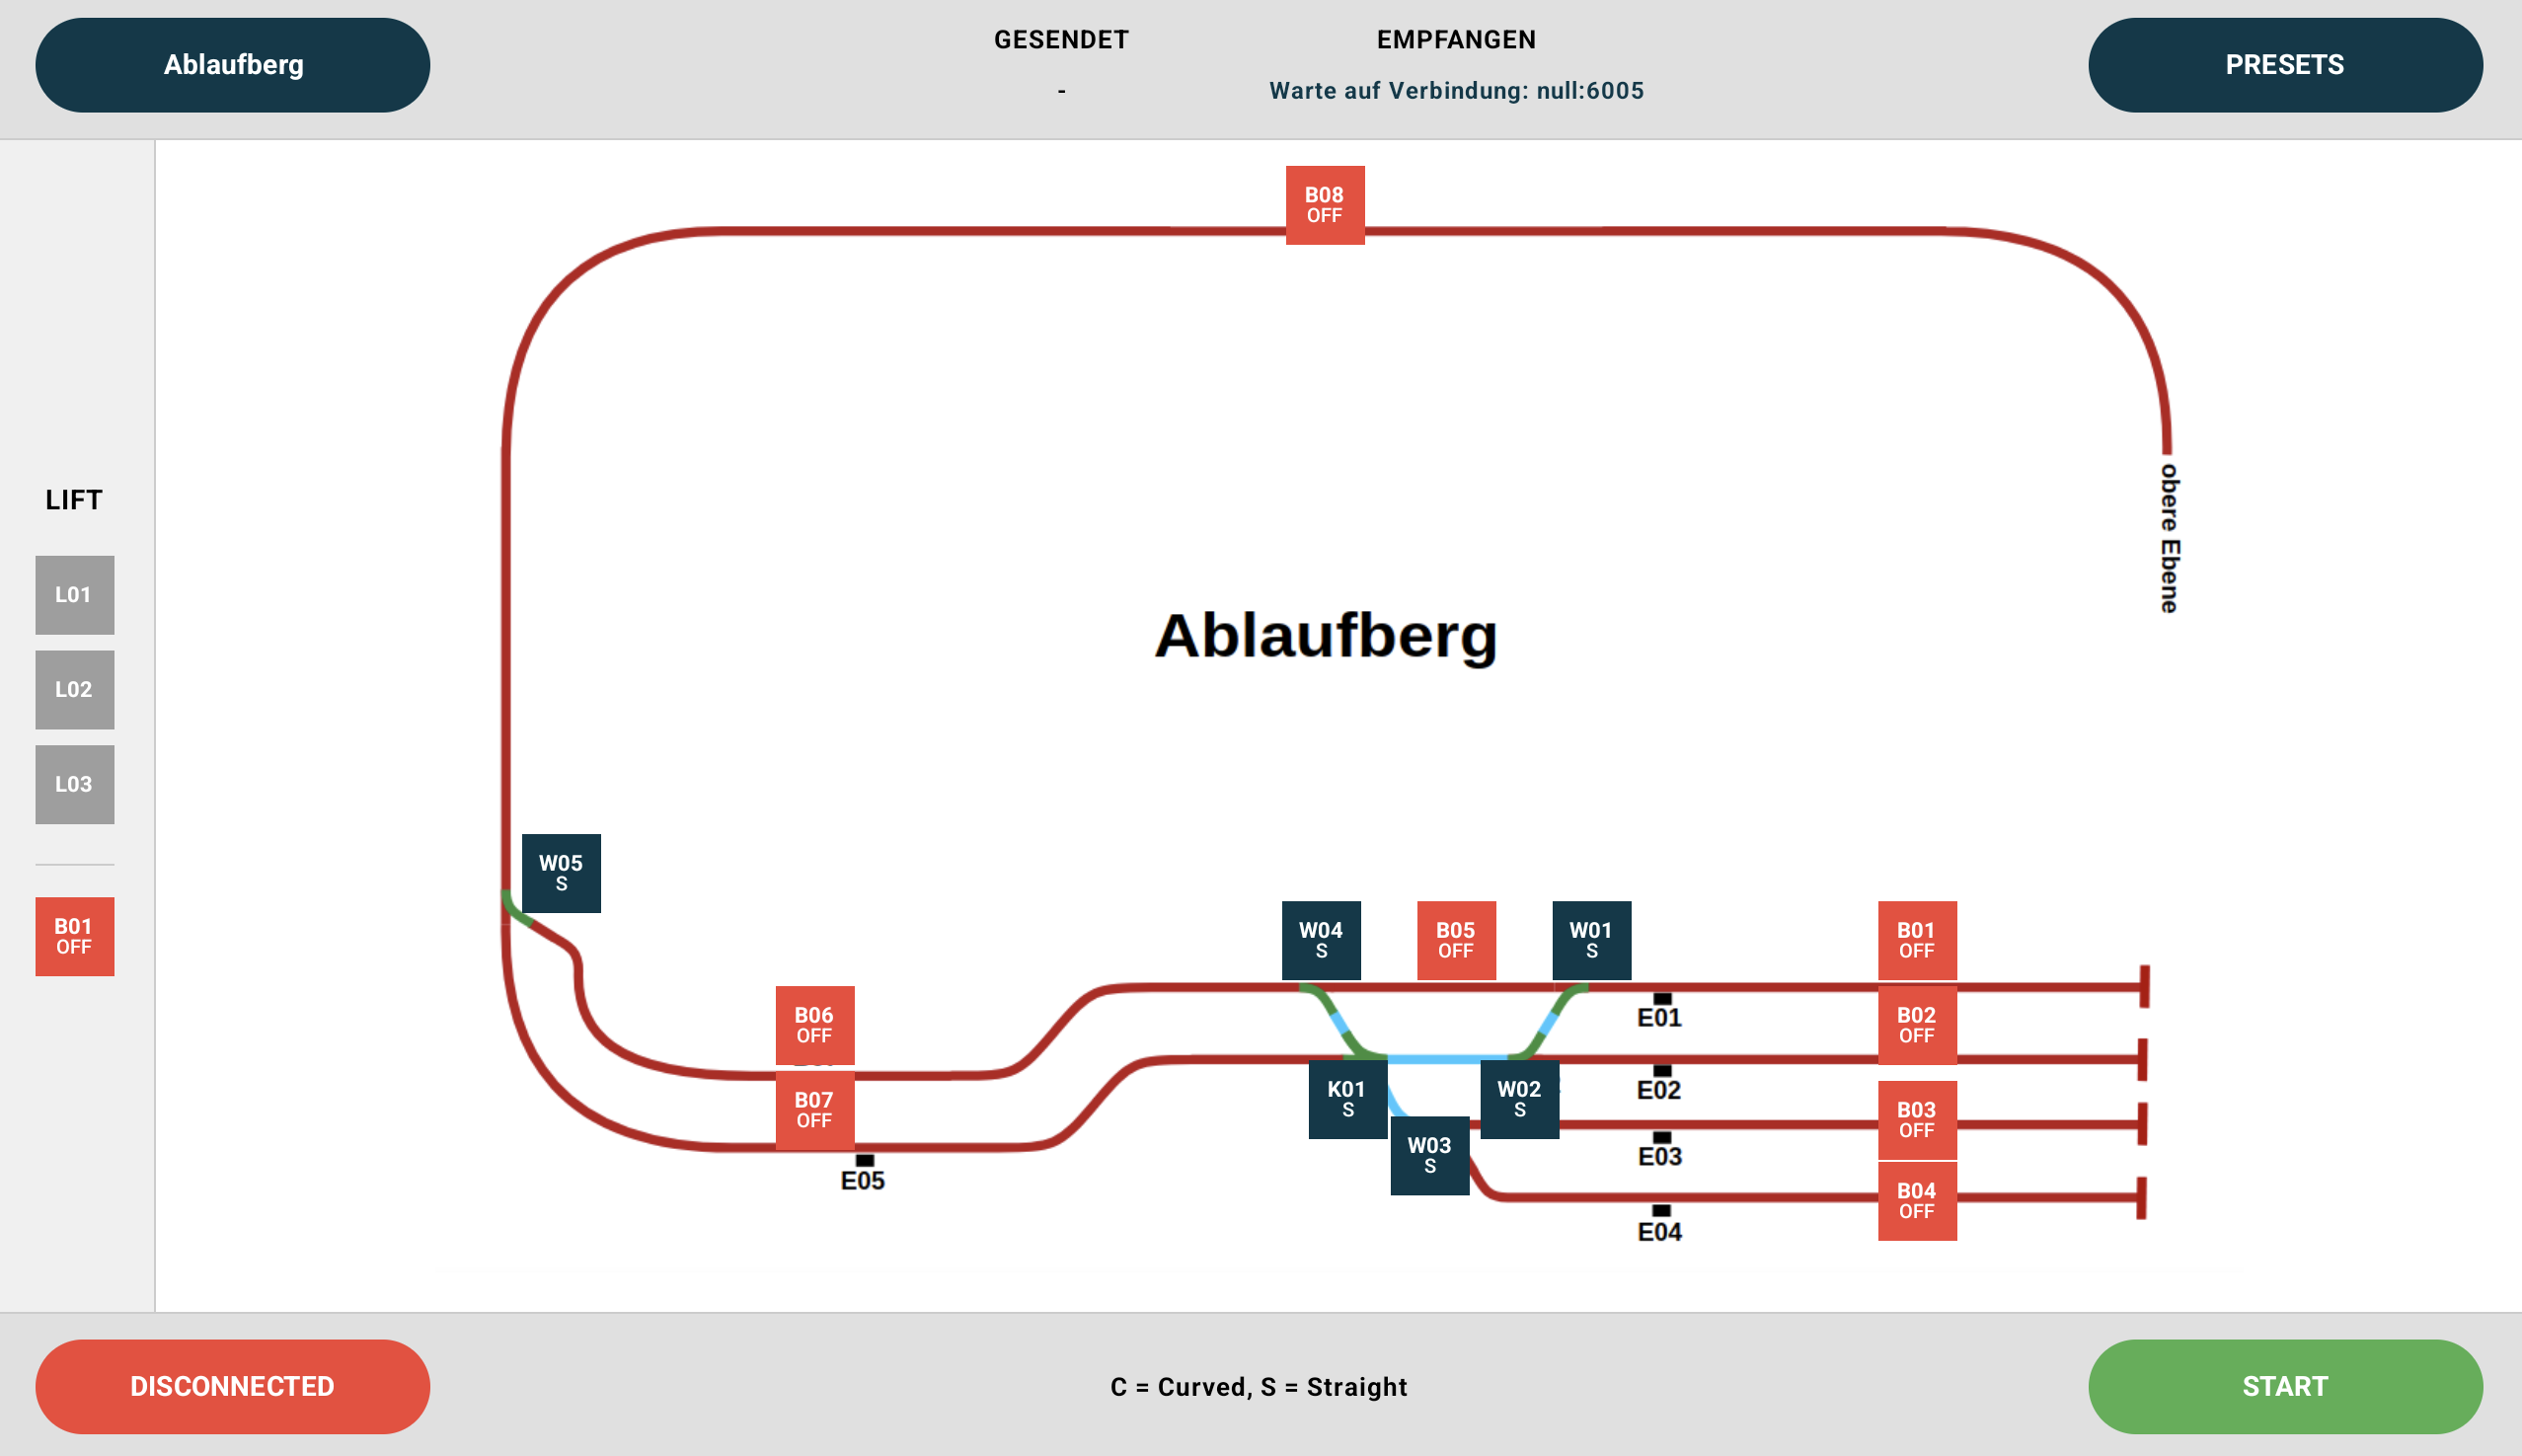
\includegraphics[width=0.9\textwidth]{App.png}
    
    \caption{Benutzeroberfläche in der Ansicht Ablaufberg.} 
    \label{fig:ui_ansicht}    
\end{figure}

\subsubsection{Layout-Struktur und permanente Navigation}
Der Header-Bereich bündelt zentrale Informationen und Navigationsmöglichkeiten. Ein zentrales Element ist das Dropdown-Menü, welches über die Liste \texttt{levels} die Auswahl zwischen dem Ablaufberg, der oberen Ebene und der mittleren Ebene ermöglicht. Flankiert wird dieses Menü von einer Statusanzeige, die über die Zustände \texttt{statusSent} und \texttt{statusReceived} den aktuellen Netzwerkverkehr visualisiert. Der Preset-Button ist zum jetzigen Stand lediglich ein Platzhalter.
Im zentralen Inhaltsbereich wird eine \texttt{Row} verwendet, um die Methode \texttt{LiftControl} als permanent sichtbare Seitenleiste am linken Rand zu fixieren. Diese Komponente erlaubt dem Nutzer den schnellen Zugriff auf die Ebenenwahl des Lifts (L01 bis L03) sowie die Schaltung des spezifischen Lift-Streckenblocks B01, unabhängig davon, welcher Gleisplan gerade im restlichen Bereich angezeigt wird.

\subsubsection{Interaktive Komponenten und visuelles Feedback}
Die Darstellung der Gleisanlagen nutzt die Methoden \texttt{Ablauf\-berg}, \texttt{Mittlere\-Ebene} und \texttt{Obere\-Ebene}, welche die jeweiligen Hintergrundgrafiken laden und mit interaktiven Elementen überlagern. Für die Steuerung kommen die wiederverwendbaren Komponenten \texttt{Track\-Block} und \texttt{Track\-Switch} zum Einsatz. Ein \texttt{Track\-Block} zeigt neben der ID den aktuellen Zustand (ON/OFF) an und ändert seine Hintergrundfarbe reaktiv basierend auf der \texttt{block\-States}-Map von Rot (inaktiv) zu Grün (aktiv). Analog dazu signalisiert ein \texttt{Track\-Switch} den Weichenzustand durch Beschriftung (S für Straight, C für Curved) und einen Farbwechsel zwischen Dunkelblau und Orange. Diese direkte visuelle Kopplung an die zentralen Zustands-Maps ermöglicht dem Nutzer eine sofortige Kontrolle über die registrierten Schaltvorgänge in der App.

\subsubsection{Systemstatus im Footer}
Der Footer schließt das Interface ab und enthält die Bedienelemente für die Gesamtfunktion. Die Farbe des Verbindungs-Buttons wird direkt durch die Zustände \texttt{is\-Connected} und \texttt{is\-Connecting} gesteuert, wodurch der Nutzer zwischen einem aktiven (Grün), einem im Aufbau befindlichen (Orange) oder einem getrennten (Rot) Netzwerkstatus unterscheiden kann. 

Daneben signalisiert der Start/Stop-Button farblich den aktuellen Sicherheitsmodus der Anlage, welcher über den \texttt{is\-Emergency\-Stop\-Active}-Status gesteuert wird. Eine ergänzende Legende im rechten Bereich des Footers informiert den Anwender zudem über die Bedeutung der Weichenkürzel, was die Bedienbarkeit der Software zusätzlich unterstützt.



\subsection{Bedienung der App}
Die Bedienung der App ist als geführter Prozess konzipiert, der den Anwender durch logische Abfolgen vor Fehlbedienungen schützt.

\subsubsection{Verbindungsaufbau und Synchronisation}
Der Betrieb beginnt mit der Herstellung der Netzwerkverbindung. Durch Betätigen des Verbindungs-Buttons im Footer initiiert der Nutzer den UDP-Broadcast. Während der Button von Rot auf Orange springt („Connecting“), wartet das System auf die Rückmeldung der Steuerrechner. Sobald die Verbindung stabil etabliert wurde und die Statusanzeige auf Grün wechselt, führt die App im Hintergrund automatisch eine Synchronisation der Weichenstellungen durch. Dieser Vorgang ist für den Anwender durch das mechanische Schalten der Hardware akustisch wahrnehmbar. Damit ist sichergestellt, dass die physische Anlage exakt der Softwarevorgabe entspricht.

\subsubsection{Fahrwegvorbereitung im Stillstand}
Nach erfolgreichem Verbindungsaufbau befindet sich das System automatisch im Sicherheitsmodus (Not-Aus aktiv). In dieser Phase kann der Nutzer über die Ebenenauswahl im Header zu den gewünschten Abschnitten navigieren. Durch Tippen auf die Weichen-Symbole (S/C) stellt der Anwender seinen Fahrweg zusammen. Da in diesem Modus noch keine Spannung an den Gleisblöcken anliegt, können Weichenstellungen gefahrlos verändert werden, ohne dass Züge unkontrolliert anfahren. Interaktionen mit den Streckenblöcken werden in dieser Phase lediglich in der App „vorgemerkt“, die Buttons ändern zwar ihre Farbe, die physische Anlage bleibt jedoch stromlos.

\subsubsection{Freigabe und Fahrbetrieb}
Sobald der Fahrweg vorbereitet ist, wechselt der Nutzer durch Betätigen des „Start“-Buttons im Footer in den Betriebsmodus. In diesem Moment werden alle zuvor in der App gesetzten Block-Zustände gesammelt an die Hardware übertragen. Die Anlage ist nun scharf geschaltet. Der Anwender kann jetzt die Züge durch Schalten der Streckenblöcke (ON/OFF) steuern. Das visuelle Feedback in der UI – der Wechsel zwischen Rot und Grün – dient dabei als direkte Bestätigung für den aktiven Stromfluss im jeweiligen Gleisabschnitt.

\subsubsection{Vertikaler Ebenenwechsel und Lift-Steuerung}
Für den Wechsel zwischen den physischen Ebenen nutzt der Bediener die permanente Lift-Steuerung am linken Bildschirmrand. Da diese Komponente unabhängig vom gewählten Gleisplan eingeblendet bleibt, kann der Nutzer den Lift jederzeit auf eine der drei Ziel-Ebenen (L01–L03) schicken. Sobald der Lift seine Position erreicht hat, kann der auf dem Lift befindliche Streckenblock (B01) aktiviert werden, um den Zug in die neue Ebene ein- oder ausfahren zu lassen.

\subsubsection{Sicherheit und Beendigung}
Sollte während des Betriebs eine kritische Situation auftreten, ermöglicht der zentrale Not-Aus-Button im Footer jederzeit die sofortige Rückkehr in den Sicherheitsmodus, wodurch alle Streckenblöcke unverzüglich stromlos geschaltet werden. Zum ordnungsgemäßen Beenden der Sitzung trennt der Nutzer die Verbindung über den Verbindungs-Button. Ein besonderes Sicherheitsmerkmal ist der automatische Abbruch. Sollte der Nutzer die App während des Fahrbetriebs verlassen oder minimieren, löst die Software selbstständig einen Notstopp aus, um die Anlage vor unbeaufsichtigten Bewegungen zu schützen.


\section{Evaluation}
Im Rahmen der Evaluation wurde die entwickelte Steuerungssoftware einem umfassenden Praxistest an der Modellanlage unterzogen. Ziel war es, die theoretischen Konzepte der Software-Architektur sowie die Implementierung der Sicherheitsmechanismen unter realen Betriebsbedingungen zu validieren.

\subsubsection{Funktionale Validierung und Konsistenz}
Ein zentraler Aspekt der Evaluation war die Überprüfung der App als alleiniger Zustandsverwalter (Single Source of Truth). In den Testläufen konnte bestätigt werden, dass die initiale Synchronisation über die Funktion \texttt{forceSyncSwitches()} zuverlässig arbeitet. Der Anwender erhält durch das mechanische Schalten der Weichen eine unmittelbare akustische Rückmeldung, wodurch die Konsistenz zwischen der digitalen Map und der physischen Anlage sichergestellt wird. Die künstliche Verzögerung von 500ms zwischen den UDP-Paketen erwies sich als effektiv, um Paketverluste, kein Fehlverhalten der Weichen und eine lückenlose Abarbeitung der Befehle durch die Steuerrechner zu gewährleisten.

\subsubsection{Überprüfung der Sicherheitsmechanismen}
Die mehrstufige Sicherheitslogik wurde gezielt auf ihre Belastbarkeit geprüft. Der implementierte Watchdog trennte die Verbindung in den Testreihen zuverlässig, sobald die Netzwerkverbindung künstlich unterbrochen wurde oder die Antwortzeiten der Hardware das definierte Zeitfenster von 25 Sekunden überschritten. Besonders hervorzuheben ist die Reaktivität des automatischen Nothalts: Das Auslösen der \texttt{onPause}-Methode beim Minimieren der App führte ausnahmslos zu einer sofortigen Deaktivierung aller Streckenblöcke. Damit wurde das Ziel erreicht, die Anlage auch bei unvorhergesehenen Nutzerereignissen in einen sicheren Zustand zu versetzen.

\subsubsection{Bedienbarkeit und Responsivität}
Die Evaluation des Bedienkonzepts bestätigte den Nutzen der zweistufigen Freigabelogik. Durch die Trennung von Fahrwegvorbereitung und Fahrbetrieb konnten Fehlbedienungen, wie das versehentliche Anfahren von Zügen bei falsch gestellten Weichen, erfolgreich vermieden werden. Die responsive UI-Architektur wurde auf verschiedenen Endgeräten emuliert. Hierbei zeigte sich, dass das System der relativen Koordinaten die interaktiven Steuerelemente präzise auf den Gleisplänen verankert, unabhängig von der jeweiligen Displayauflösung. Die permanente Sichtbarkeit der Lift-Steuerung am linken Rand erwies sich in der Praxis als großer Vorteil für die Effizienz des Ebenenwechsels, da keine Menüwechsel erforderlich waren, um die vertikale Achse der Anlage zu kontrollieren.

\subsubsection{Zusammenfassung der Ergebnisse}
Zusammenfassend lässt sich festhalten, dass die Software alle gestellten Anforderungen erfüllt. Die gewählte Architektur bietet eine stabile und wartbare Basis für den Testbetrieb. Die Kombination aus reaktiver Zustandsverwaltung in Jetpack Compose und der strikten Sicherheitslogik im Hintergrund ermöglicht eine intuitive, aber dennoch kontrollierte Steuerung der komplexen Modellanlage. Für zukünftige Erweiterungen bietet die modulare Struktur der App zudem ausreichend Spielraum, um weitere Anlagenteile oder automatisierte Abläufe ohne grundlegende Änderungen am Systemkern zu integrieren.


\end{document}
